\documentclass[../OAE-SPEC-MAIN.tex]{subfiles}

\title{Cells and Links}

\begin{document}

\chapter{Cells and Links}\label{sec:cells-and-links}
%\marginnote{The  biggest problem with communication is the illusion that it has happened. [George Bernard Shaw?]}

\CELLs and \LINKs are  fundamental elements. \LINKs are \emph{bipartite} causal relationships connected over physical cables (backplanes, coax, fiber). 






\section{Cells}

A \CELL is not merely a general-purpose computer. It is a reactive, self-contained participant in a global program. Each \CELL holds local state, executes transactions, and engages in atomic communication with its neighbors. It participates in reversible protocols, encodes causal histories in state transitions, and makes decisions based on local information while remaining consistent with a global ordering.

\CELLs maintain a timebase, manage a local execution queue, and process both incoming transactions and local tasks. Their execution model is event-driven and transactional, but grounded in physical links—each \CELL’s “world” is bounded by the links it can reach.

Crucially, \CELLs are interchangeable. There is no distinction between a compute node, a storage node, or a network switch. Each \CELL contains a portion of all three. The specialization comes from programmatic configuration and emergent behavior, not fixed hardware roles.

\subsection{Failure Modes}

\CELLs fail in bounded ways. The execution environment guarantees that failure is:
\begin{itemize}
\item \textbf{Local}: A failing \CELL does not compromise its neighbors.
\item \textbf{Detectable}: Liveness and responsiveness can be externally verified through link activity and expected transactions.
\item \textbf{Reversible}: As much as possible, computation and state changes at a \CELL can be rolled back or isolated through transaction lineage and local journaling.
\end{itemize}

Failures may be:
\begin{itemize}
\item \textbf{Crash-fail}: power loss, watchdog-triggered resets, or thermal shutdowns.
\item \textbf{Byzantine}: misbehavior due to bitflips, radiation events, or malicious actors. These are constrained by cryptographic and causal transaction tracking.
\item \textbf{Soft}: overloaded slots, or clock skew outside tolerances.
\end{itemize}

The system design assumes failure. What matters is how neighboring \CELLs detect, isolate, and route around the failure using only local knowledge.





\section{Links}

A \LINK is a bidirectional tunnel-element; an autonomous communication entity between  \emph{two} \texttt{CELLs}. Think of  \LINKs as compute elements with their own autonomous and independent failure domain. Physically, the \LINK comprises the cable and SerDes' on both ends to form a self contained execution environment.

\LINKs are autonomous in that they maintain state: pending transactions, reversibility buffers, sequence tracking, and retry logic. They mediate causality between two \CELLs and enforce atomic delivery guarantees over physical media that may be noisy, lossy, or delayed.

A healthy \LINK behaves like a lock-free memory bus: it transmits events, ensures ordering, and preserves invertibility for transactional safety. But unlike a memory bus, it must contend with delay, noise, and the limits of the speed of light. Its job is to conceal those imperfections behind a deterministic, reversible interface.

\LINKs are not passive -- they can be reset, throttled, or even reprogrammed in the field. They may expose telemetry, accept diagnostic pings, or reconfigure modulation in response to environmental conditions.

\subsection{Link Utilities}

Physical \LINKs Implement utilities that used to be in logical link domains above L2: in  L3, L4, or L7;  composed into an abstraction of logical links. This is an illusion. If the pairing of Shannon information is thrown away at layer 2, it cannot be recovered in higher layers. This is addressed in more detail in the \emph{Key Issue} section below.

An example\sidenote[][-40mm]{Synchronization of timing domains in computers generally start from the processor clock on the motherboard, and fan out through the logic into the I/O subsystems. \IUI lives in the LINK between two \emph{independent} computers, and although it receives information from either side, it is not synchronized with either side. This independent asynchronous domain (already exploited in the HFT Industry) -- enables failure independence and atomicity.} \LINK utility is \emph{The I Know That You Know That I Know} (\texttt{TIK\hspace{1pt}TYK\hspace{1pt}TIK}) property; which  enables us to address some of the most difficult and pernicious problems in \emph{distributed systems} today. 

Another example \LINK utility is \emph{Indivisible Unit of Information} (\texttt{IUI}). Unlike \emph{replicated} state machines (RSM's) used throughout distributed applications today, \LINKs \emph{are} state machines: the two halves of which maintain \emph{shared state} through hidden packet exchanges.  When a local agent or actor is ready, the\IUI protocol transfers \emph{indivisible}
tokens across the LINK to  the other agent, \emph{atomically} (all or nothing)
\sidenote[][-10mm]{\LINKs are \emph{exquisitely} sensitive to packet loss. This is intentional: we turn the \href{https://groups.csail.mit.edu/tds/papers/Lynch/jacm85.pdf}{FLP} result \emph{upside down}, and use ``a single unannounced process death'' to guarantee the atomic property for\IUI.}. 
 
\noindent  \texttt{TIK\hspace{1pt}TYK\hspace{1pt}TIK} and \IUI properties are mathematically \emph{compositional}. 

What's necessary is an \emph{entanglement} between state machines -- locking them together silently in normal operation, and failing locally at the first failure.  The entanglement cannot be recovered if information from events can disappear. This is the only solution to the problem in the  latency--disconnection ambiguity [Ref: CAP Theorem Tradeoffs]. To put it in terms an engineer can internalize, a system that fails instantly, can heal immediately.


\subsection{Failure Modes}

The \emph{shared state} property %of the bipartite \LINK object
is strengthened by mechanisms to recover from each type of failure. The more types of failures, the more complex and intractable this becomes. \LINKs are independent failure domains, with (effectively) one failure hazard: \emph{disconnection} \sidenote[][-0mm]{In any physical system it is possible to drop packets, it will be much rarer but it is still possible. \LINKs can recover from individually dropped or corrupted packets, and \emph{shared state integrity} can be maintained through out the successive reversibility recovery -- back to the equilibrium state.}; which is straightforward to recover from.








\section{Initial Discovery}

 \begin{marginfigure}
        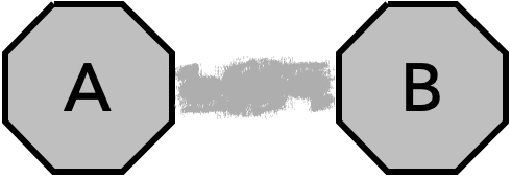
\includegraphics[width=\linewidth]{../../FIGURES/Bipartite-discovery.pdf}
  \caption{A Link yet to be discovered, or a flakey link that need to be repaired}
      \vspace{12pt}
\end{marginfigure}


\CELLs discover connections $\exists$xist on \emph{each} of their ports. For connections that  once existed (which may have been remembered from previously being powered up), we will find it \emph{impossible} to tell whether we are being woken up for the $1$st time, or the $N$th time*. \marginnote{*Sleeping Beauty paradox: Veritasium:  \href{https://youtu.be/XeSu9fBJ2sI?si=Nl70HKeFJT1Rlexb}{The Most Controversial Problem in Philosophy}}

\texttt{Alice} and \texttt{Bob} have no knowledge of each other prior to being powered up for the first time. They discover each other by sending and responding to \texttt{BEACON}s on each of their 8 ports $\{n,ne,de,se,ds,sw,dw,nw\}$. \texttt{BEACON}s are questions: ``is anyone there?'' They assume  neighbor \CELLs have SerDes' that can send \& receive @ 25Gb/s (defined by local clocks, in their frame of reference). Photon cavities (copper and fiber) are expected to be in a fixed frame of reference relative to the \texttt{SELF} \CELL.  Mobile entities may need to adjust this expectation based on the range of doppler shifts expected by \CELLs in motion, for example, in moving vehicles, \texttt{cars}, \texttt{planes}, and \texttt{spacecraft}.


Alice sends \texttt{BEACON}s with an exponential backoff: every $1\mu s$, $2 \mu s$, $4 \mu s$, 8 $\mu s$, etc. The  policy for a maximum interval  is determined by the environment, e.g. within a datacenter, one might wish to send  \texttt{BEACON}s every second, whether you need to or not.  This  represents a balance between infrastructure liveness and needless energy dissipation.


Single Links are subject to \emph{partial} or \emph{total} failure. Although networks use the word  `partition', for example in the CAP Theorem\cite{CAP}, this concept is inappropriate except in the single \LINK case, when there's no communication with the other side; the  \emph{causal %Ref David Deutch
 universes**\marginnote{\emph{**Quantum Compatible Interpretation}}} are now isolated from each other.
 
 
 
 
 
 
 
 
\section{It takes Two to Tango, and Three to Party}

%\subsection{Alice, Bob, and Carol with 3 LINKs}

Because a single link between Alice and Bob can be causally disconnected by real-world, permanent or intermittent failures, an alternative: statistically--independent--failure--path is necessary, to recover from \LINK Failures.  % ADD MODAL LOGIC necessary, etc.
This is the heart of the  Æ \texttt{ATOMICITY} claim:   A local (one hop \LINK) \texttt{TRIANGLE}  is the minimum necessary.  See TRIANGLE Clocks later in this specification.

 \begin{marginfigure}
        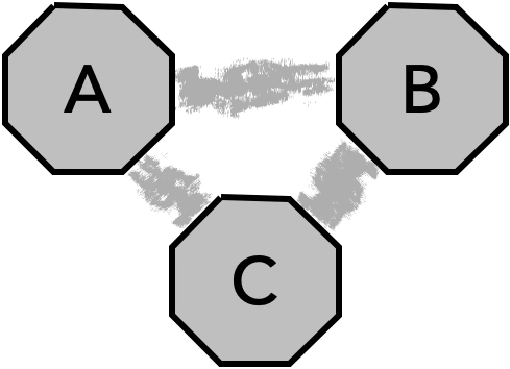
\includegraphics[width=\linewidth]{../../FIGURES/Tripartite-discovery.pdf}
  \caption{It takes three to party.  Links need an alternate path. This won't work over a Switched (Clos) Network.  
}
 %   \caption{A-B-C Flakey.pdf}
    \vspace{16pt}
\end{marginfigure}


%\subsection{\LINKs are Flakey}

 \begin{marginfigure}
      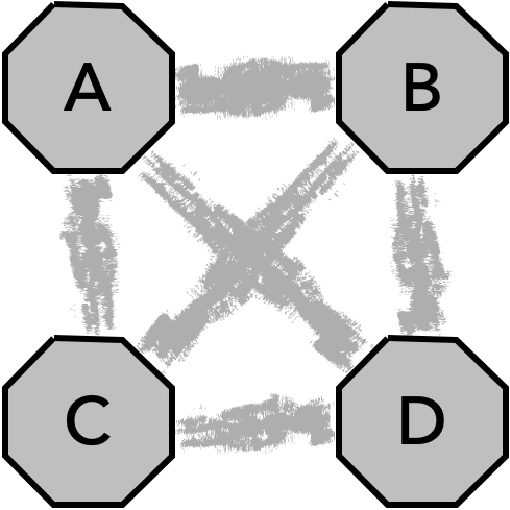
\includegraphics[width=\linewidth]{../../FIGURES/Quadpartite-discovery.pdf}
  \caption{2 x 2 =4  connected nodes with 6 flakey LINKs. Any one of which may be working in both directions: $\{11\}$, only one direction: $\{01\}$ or $\{10\}$, or \emph{not}-working in  \emph{both} directions: $\{11\}$. For 4 nodes, there are $\frac{(n(n-1)}{2} = 6$. With 4  \emph{reliability configurations} on each \LINK $\{00,01,10,11\}$ This gives us ONE correct (all links working correctly) and  $4^6-1 = 4095$ possible failure modes.}%\marginnote{permutations or combinations?} 
   \vspace{10pt}
\end{marginfigure}



\section{Fault Model}

\marginnote{
Benefits include (i) Shorter packets and more effective use of bandwidth, (ii) more complete coverage of possible failure modes. (iii) Guarantees at least the first slice is perfect (matches what the transmitter knows they sent). }

AE-Links present two major differences to the conventional FEC thinking in today's Ethernet, which exploits the physics from 25Gb/s to 1.6Tb and beyond:

\begin{description}
\item [Perfect Information Transfer (PIF)] Æ-Links use Back-to-Back (B2B) Shannon Links, where the receiver returns the first 8-byte slice of each 64-Byte packet to the transmitter. This ``here is what I heard you say" ( Perfect Information Transfer (PIF)\cite{Paper from Garner}

\item [Epistricted Registers (EPI)] Borrowing from the Spekkens' toy model for quantum entanglement, we narrow down the possible entangled states to a vastly smaller set of possibilities, using the model described in Quantum Ethernet\cite{Quantum Ethernet}.
\end{description}



\subsection{Failure Model}

Consider a network of \(n\) nodes connected by undirected Ethernet
links.  Each link can be in one of four independent reliability
states,
\marginnote{
\[
\Sigma=\{00,01,10,11\},
\]}
where \(11\) means the link works in both directions, \(10\) or
\(01\) means it works in only one direction, and \(00\) means it
is broken in both directions.

%\subsection{Link count}

Because every node may attach to at most eight neighbours (an
\emph{octavalent} mesh), the number of physical links is
\marginnote{
\[
L(n)=\min\!\bigl\{\tbinom{n}{2},\,4n\bigr\}
=
\begin{cases}
\binom{n}{2}, & n\le 9,\\[6pt]
4n,            & n\ge 9.
\end{cases}
\]}

%\section{Reliability configurations}

Each link chooses a state from \(\Sigma\) independently, so the total
number of configurations is \(4^{\,L(n)}\).
Exactly one of these is fully healthy (all links in state \(11\)), hence
\[
\text{FailureModes}(n)=4^{\,L(n)}-1.
\]

\subsection{Enumerated results for \(2\le n\le20\)}

%\begin{table}[ht]
\begin{margintable}
\centering
\begin{tabular}{@{}rrr@{}}
\toprule
\(n\) & \(L(n)\) & Failure modes \(4^{\,L}-1\)\\
\midrule
 2 &  1 & 3\\
 3 &  3 & 63\\
 4 &  6 & 4\,095\\
 5 & 10 & 1\,048\,575\\
 6 & 15 & \(1.074\times10^{9}\)\\
 7 & 21 & \(4.398\times10^{12}\)\\
 8 & 28 & \(7.206\times10^{16}\)\\
% 9 & 36 & \(4.722\times10^{21}\)\\
%10 & 40 & \(1.209\times10^{24}\)\\
%11 & 44 & \(3.095\times10^{26}\)\\
%12 & 48 & \(7.923\times10^{28}\)\\
%13 & 52 & \(2.028\times10^{31}\)\\
%14 & 56 & \(5.192\times10^{33}\)\\
%15 & 60 & \(1.329\times10^{36}\)\\
%16 & 64 & \(3.403\times10^{38}\)\\
%17 & 68 & \(8.711\times10^{40}\)\\
%18 & 72 & \(2.230\times10^{43}\)\\
%19 & 76 & \(5.709\times10^{45}\)\\
%20 & 80 & \(1.462\times10^{48}\)\\
\bottomrule
\vspace{8pt}
\end{tabular}
\caption{Failure‑mode counts for an octavalent mesh with \(n\) nodes.}
\vspace{12pt}
\end{margintable}
%\end{table}

\section{Set Reconciliation of Shannon Slots}

The first claim is that a finite and enumerable number of  `slots' exist on both sides of the LINK. In conventional Ethernet, once these slots are exhausted (with for example, a timeout and retry, the XPU CELLS (SmartNICs) on both sides of the LINK must evict (erase) the information on one side and then the other. This `loss of Koherence' is the central problem of Distributed Systems.  From an information theoretic (Back to Back Shannon channel) perspective, this precipitates a `smash and restart (SAR) of the Shannon Information --  the loss of `pairing' of information. This is described in more detail in the specification of back-to-back Shannon Pairs.

Timeouts and Retries are the root of all evil.  Once a Timeout Storm occurs, in a switched network, the distributed systems in the Host processor are all broken. Unless RELIABILITY (maintenance of Shannon Link Pairing),  the `global' illusion of event ordering in distributed systems will be lost, and corruption will occur.  This is why queue-pairs work in Infiniband/RDMA. This is why information pairing is essential, in Tandem's Process Pairs, and RDMA's Queue pairs.

The whole point of this specification is to engineer a solution, where Shannon-pairing is never lost, but if it is, a TRIANGLE healing occurs locally, without the need to depend on a switched or router to discover and  `reconverge' their routing tables, to re-establish the point to point connections over a different paths in the network.  

The main mechanism to do this is to make the Æthernet Link maintain Koherence, and when loss occurs, a 3rd party (The Triangle relationship) can recover with local information only. This makes XPU/SmartNICs, where the recovery algorithms (healing the tree) occur locally, instead of waiting for the switched or routed packets (in a separate switched network.

The original Ethernet was unreliable. This was a mistake. Infiniband already proved this, and succeeded both in the trust system archicitcts have in the far greater. The unique contributions of this specification is to go (far) beyond Infiniband's discovery, and recognize the fundamental simplifications and benefits that Infiniband (and Token Ring,  Fibrechannel, and Sonet), in creating `Race-Free' protocols, where distributed systems can guarantee, not just the `ordering of events', but the guarantee of recovery of transactional loss in when failures occur in the middle of, say, a 2 Phase Commit. 

Æthernet (Atomic Ethernet) guarantees that Shannon Pairing is never lost, and if a link breaks, that the Coordinator (Charlie, Carol, Chief) can recover with TRIANGLE Relationships, far faster than any protocol stack in the host processor, or in the RMDA message relationships, but then add, on top of this a true `atomic' relationship between CELLS (nodes) in a distributed system.

The original Ethernet [ref] was designed around a notion of slots. These were `time slots' on an imaginary timeline that each node on the Ethernet Cable, could manage in a half-Duplex way.  The new notion is to replace this with circulating tokens, where each slice is independently acknowledged, providing a guarantee of delivery to the NEXT hop in the network.

This is achieved with 1PC (one phase commit), where each Ethernet Packet (eight slices) are fully acknowledged in each link. The generalization of this is to explicitly manage Shannon slots (data structures on each side of the link) to maintain Koherence, even when the link fails (in one direction, the other direction, or in both directions at once).

This can be done (as in Fibrechannel)  by arranging the `interaction protocol' to guarantee the pairing of events, and not resort to Timeout and Retry (TAR), which causes cascade failures in networks, both large and small.

This is achieved with the Link Protocol employing the Alternating Bit protocol, and adding the Bill Lynch ABP reconciliation, with two or more bits instead of the individual 1 bit of alternation, which required a round trip to guarantee Shannon Slot Pairing.


\section{FAQ}

Q1 (Alan) What problem are you addressing in the scouting writeup?  If it’s discovering routes, it’s not clear to me that ant or bees or even both together do full discovery of the network.  In what way are they better than the flooding algorithm I used?

A1 This is how to achieve `Scale-Independence' We eliminate the need for   every node  to do a `full discovery' of the network, which is what a flooding algorithm would do.  ANTs and BEEs explicitly do not do ``Global" routing. This is an extra way to limit the size of the secure enclave, and not have it able to connect to the outside world.  

\end{document}
